%%%%%%%%%%%%%%%%%%%%%%%%%%%%%%%%%%%%%%%%%%%%%%%%%%%%%%%%%%%%%%%%%%%%%%%% 
%%%%%%%%%%%%%%%%%%%%%%%%%%%%%%%%%%%%%%%%%%%%%%%%%%%%%%%%%%%%%%%%%%%%%%%% 
\begin{frame}[fragile=singleslide]
  \frametitle{Hands-On 8 : Euler equation solver}

  \hypertarget{handson8}{}
  \begin{itemize}
  \item Original serial code: \texttt{\$HOME/patc\_kokkos/code/miniapps/euler2d\_serial}
  \item See additionnal slides in source directory about CFD numerics
  \item \textcolor{red}{\bf Activity 1: Porting code to kokkos:} the serial version has been partially ported to kokkos; fill the TODOs to complete.
  \item \textcolor{darkgreen}{\bf Activity 2: Build / run / mesure performance} of the kokkos solution (directory \texttt{euler2d\_kokkos\_solution}). Try to plot the OpenMP weak scaling on Power8.
  \item {\bf How much faster is the GPU version (Pascal P100) versus the Power8 ?}
  \end{itemize}
  
  \begin{center}
    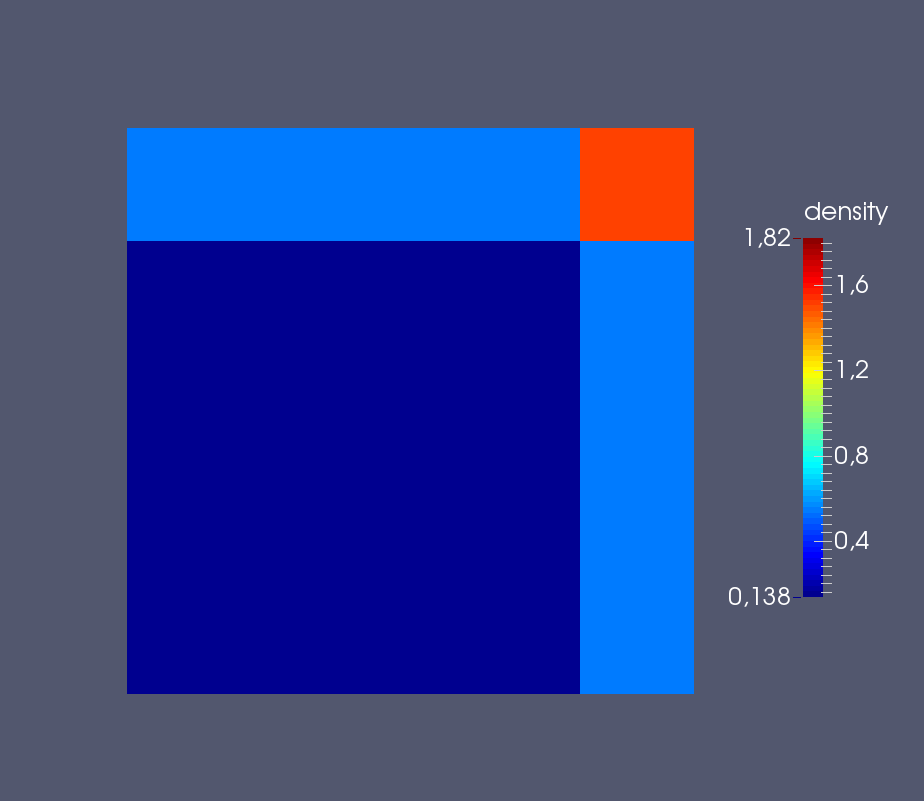
\includegraphics[height=3.0cm]{../euler/images/riemann/riemann_1}
    \hspace{0.1cm}
    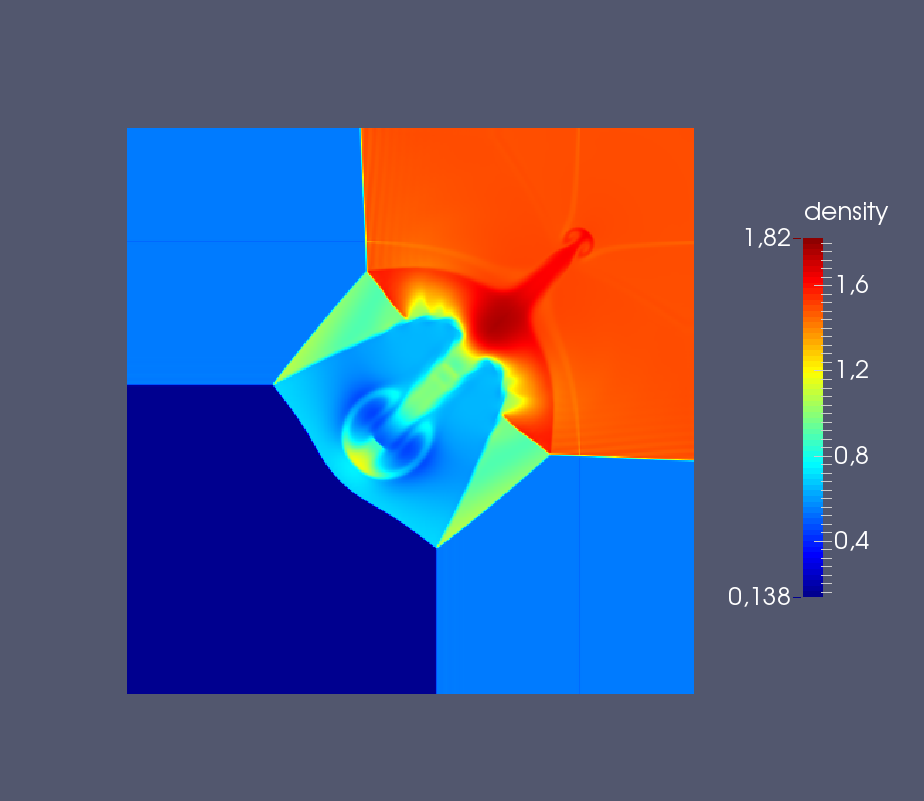
\includegraphics[height=3.0cm]{../euler/images/riemann/riemann_2}
  \end{center}


\end{frame}
